\chapter{Reinforcement Learning}
\begin{quotation}
\noindent ``\emph{quote}''
\begin{flushright}\textbf{auteur, date}\end{flushright}
\end{quotation}

\vspace*{0.5cm}

\section{Machine Learning}
One could trace back the birth of the machine learning idea to Alan Turing's 
seminal paper, \textit{Computing Machinery and Intelligence} 
\cite{turing1950computing}. Although the computer science context around his
work was largely inexistent (at least compared to today), Turing already felt
the need to think of ways to transcend the fixed set of rules a computer had
to interpret and execute. As computer science grew, and as the field of
artificial intelligence went through its ebbs and flows throughout the years,
machine learning evolved from an idea to a prolific field of research, and
some of its topics saw massive application into real world domains.\\

The most popular and widely used machine learning algorithms and techniques
usually come from what we call supervised and unsupervised machine learning.
The broad goal of supervised machine learning is to find a function that maps
some input vector $x$ to some output vector $y$. One example of this would be
to try to categorise patients that either have or don't have some disease. 
The input vector $x$ could contain measurements such as blood pressure, the 
quantity of a given substance in the patient's blood, etc. The output vector
$y$ would be either $[0]$ if the patient is ill, and $[1]$ if the patient is
not.\\

If we could find a function mapping $x$ to $y$, we could predict to some
level of accuracy if a patient is ill or not by only knowing $x$. The general
algorithm for finding such a function is to define a model which has
\textit{learnable parameters}; that is values which impact the output of the
function, and to perform \textbf{training}. The process of training is to
sample one data point from a \textbf{training set}, containing pairs of input
vectors and output vectors. We then feed the input vector to our model, compare
the output that we get from the model with the output we are supposed to get,
and tune our learnable parameters so to minimise the error between the model
output and the correct output. We repeat this process, showing many samples
of the training set to our model until it reaches a good enough accuracy.

Unsupervised learning, although different from supervised learning as the
training sets usually do not have output vectors, is more about finding
structure in the dataset; but we can assume for the sake of this point that
the process is largely the same.\\

To the critical reader, unsupervised machine learning and supervised machine
learning might sound like fancy names for statistics; and one could argue that
they are indeed. Perhaps a slightly more interesting topic of machine learning
would be \textbf{reinforcement learning}. In this setting, we train an agent, 
which is situated in an environment, to perform actions that will maximise
a reward given by the environment.\\

This process works by letting the agent interact with the environment for many
sessions, until it figures out what actions, and what sequences of actions lead
to high rewards. This is the training process of a reinforcement learning agent.
One example of this is the CartPole problem \cite{barto-cartpole} where the
agent controls a cart on which a pole is balanced. The goal is to keep the
pole balanced for as long as possible by nudging the cart left or right. The
agent receives the position of the cart, the velocity of the cart, the pole
angle and the pole velocity at tip as a state observation from the environment,
and has to push the cart either left or right. The agent will first perform
randomly, but sooner or later, it will figure out how to balance the pole.\\

One common issue between all of the techniques described above is that once
training is over, the behaviour of the trained agent or model will not change
or adapt once the conditions, or some intrinsic parameters of the problem
change. If we present the CartPole agent with a pole that is twice as heavy,
or twice as long as the one it has been trained with, it will likely fail to 
balance the pole. We have taught an agent how to solve one task, but we have
not taught it to learn how to solve a task. The agent that has been trained is
not a learning agent. This thesis will explore ways to teach an agent to learn
to solve tasks.

\section{The reinforcement learning problem}
A reinforcement learning setting sees two main components interact : the agent
and the environment. The environment can be in several states which the agent
can observe (for example in the CartPole problem : the cart can be in several 
positions and have different velocities, and the pole has similar 
characteristics). In some problems, the agent might not be able to observe the
full state of the environment.\\

The agent chooses actions based on its knowledge of the state of the
environment. These actions might (and often do) alter the state of the
environment, but will also generate a reward. In the CartPole problem, the 
reward is +1 every tick the pole is above a certain angle, 0 otherwise.\\

With this simple setting, of which a diagram is shown in Figure~\ref{fig:rl},
we can design algorithms that can be trained to solve a huge variety of tasks
without ever having to include task-specific logic to the algorithm.

\begin{figure}[]
	\centering
	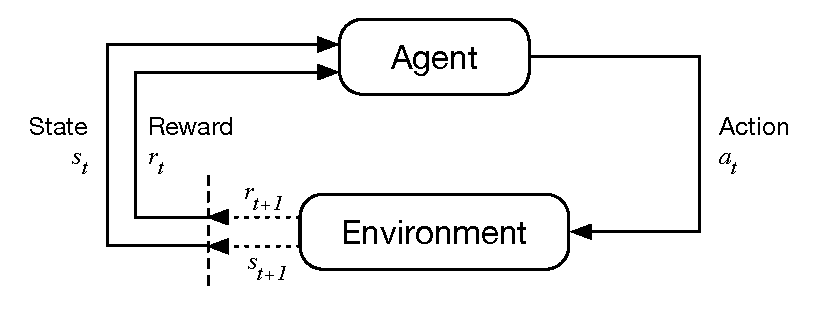
\includegraphics[width=0.65\linewidth]{fig/rl.eps}
	\caption{The setting of a reinforcement learning problem 
		\cite{suttonbarto}}
	\label{fig:rl}
\end{figure}

\subsection{Markov Decision Processes}
A reinforcement learning problem can be formally defined as a Markov 
Decision Process (MDP) \index{MDP} characterised by :
\begin{itemize}
	\item a set of states $\mathcal{S}$
	\item a set of actions $\mathcal{A}$
	\item a transition function 
		$T(s, a, s') = P(s_{t+1} = s' \mid s_t = s, a_t = a)$
	\item a reward function 
		$r(s, a, s') = \mathbb{E}
		 [r_{t+1} \mid s_t = s, a_t = a, s_{t+1} = s']$
\end{itemize}
For the rest of this paper, we will consider that the transition function is
deterministic.\\

The goal of reinforcement learning is for the agent to select, in any state it
can be in, the action that will lead it to the highest expected reward :

\begin{equation}
\mathbb{E}[r] = r_t + \gamma r_{t+1} + \gamma^2 r_{t+2}^2 + ... =
 \sum\limits_{i=0}^\infty \gamma^i r_{t+i}
\end{equation}

\noindent with the discount factor \index{discount factor} $\gamma \in [0, 1[$.
The discount factor allows one to tune the agent's behaviour on the
short-term/long-term spectrum. A discount factor $\gamma=0$ would mean that the
agent maximises its expected reward for the next transition only whereas a
discount factor close to one will favour behaviour that maximises long-term
reward, even if one action leads to a poor reward at first.\\

\subsection{Policy}
The agent uses a policy $\pi(a \mid s)$ which describes a probability
distribution over the action set $\mathcal{A}$, determining the probability of
selecting action $a_i$ from state $s_i$. This policy is 
\textbf{deterministic} if and only if :
\begin{equation}
\forall\, s \in \mathcal{S},\; \exists\, a \in \mathcal{A} : \pi(a \mid s) = 1
\end{equation}
\noindent Otherwise, the policy is \textbf{stochastic}.

\section{An example : the 2-armed bandit problem}



